\documentclass[times, utf8, diplomski]{fer}

\usepackage{booktabs}
\usepackage{float}
\usepackage{algpseudocode}
\usepackage{algorithm}

\algnewcommand{\Or}{\textbf{ or }}
\algnewcommand{\And}{\textbf{ and }}
\newcommand{\classname}[1]{\texttt{#1}}

\graphicspath{ {./images/} }
\setcitestyle{numbers}
\setcitestyle{square}

\begin{document}

\thesisnumber{2963}
\title{Razvoj i primjena biblioteke za umrežavanje višekorisničkih videoigara}
\author{Filip Nemec}
\maketitle

% Ispis stranice s napomenom o umetanju izvornika rada. Uklonite naredbu \izvornik ako želite izbaciti tu stranicu.
% \izvornik

% Dodavanje zahvale ili prazne stranice. Ako ne želite dodati zahvalu, naredbu ostavite radi prazne stranice.
% \zahvala{}

\tableofcontents

\chapter{Transport}
This chapter introduces and explains in detail the concept of a transport layer. It starts by giving an introduction to networking, explaining motivation behind a layered structure. It then discusses today's most widely used transport layers. Finally, it finishes by giving a detailed look into a custom transport layer implementation.

\section{Introduction}
Computer networking is a very complex problem. It consists of many different sub-problems, such as packet-routing, data transmission, integrity, reliability, congestion-control, flow-control and much more. In order to deal with such complexity, ISO (International Organization for Standardization)\footnote{https://en.wikipedia.org/wiki/International\_Organization\_for\_Standardization} developed OSI (Open Systems Interconnection) model\footnote{https://en.wikipedia.org/wiki/OSI\_model} in the year 1984. OSI model divides complex problem of computer networking into a structure consisting of 7 layers\footnote{https://www.geeksforgeeks.org/layers-of-osi-model/}, each layer building on top of the layer below it. Layers are defined as follows:

\begin{enumerate}
	\item \textbf{Physical layer} is responsible for transmission of raw signals between two or more physical entities. Jobs of this layer include transmission of bits, bit-rate control and support for various modes of transmission such as simplex, half-duplex and full-duplex.
	
	\item \textbf{Data-link layer} enables communication between two neighboring network nodes (devices). Basic functions of this layer include point-to-point frame transmission, error-control and data-flow control. 
	
	\item \textbf{Network layer} solves the problem of end-to-end device communication. Functions of network layer include routing (finding optimal route for data to reach its destination) and logical addressing (ability to uniquely identify a device on the computer network).
	
	\item \textbf{Transport layer} is responsible for transmission of data from process-to-process while satisfying transparency criterion. There are two types of transparencies \cite{kommre}:
	
	\begin{enumerate}
		\item \textit{Semantic transparency} whose only task it to ensure that data arrives reliably and in-order it was sent.
		\item \textit{Temporal transparency} that only focuses on delivering data as fast as possible.
	\end{enumerate}

	\item \textbf{Session layer} is responsible for establishing, maintaining and terminating connections, authentication and security.
	
	\item \textbf{Presentation layer} is responsible for encryption/decryption, compression and translation between data formats.
	
	\item \textbf{Application layer} is where all of the data is produced, processed and shown to the end-user. 
\end{enumerate}

With such layered structure, we introduced concept of \textit{abstraction}. Every layer simply uses implementation below it without the need to know how it is implemented. This gives us the ability to easily swap out implementations of different layers in the stack.


\begin{figure}[h!]
	\centering
	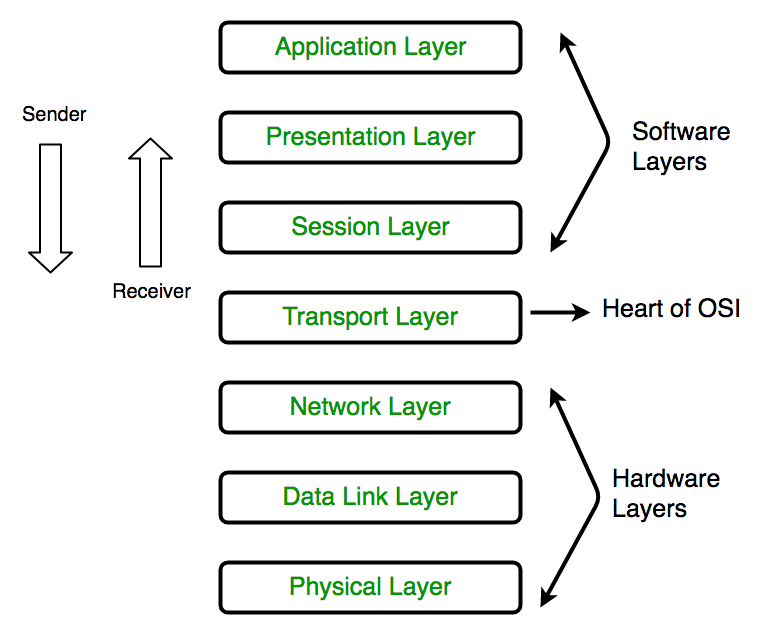
\includegraphics[scale=0.32]{OSI-model-layers}
	\caption{OSI layers, from \cite{GeeksForGeeks:OSI-model}}
\end{figure}


\section{Existing transport implementations}
Previous section mentioned the terms of semantic and temporal transparency. Consequently, there exist two different transport layer implementations, one for each transparency type. \\

The first protocol, which implements semantic transparency, is called TCP (Transmission Control Protocol)\footnote{https://datatracker.ietf.org/doc/html/rfc793}. TCP abstracts away the concept of computer network and exposes a simple interface to the user, where writing bytes is almost the same as writing to a simple binary file. \\

The second protocol, which implements temporal transparency, is called UDP (User Datagram Protocol)\footnote{https://datatracker.ietf.org/doc/html/rfc768}. UDP is a protocol that implements a thin layer of abstraction over the network layer.

\begin{figure}[h!]
	\centering
	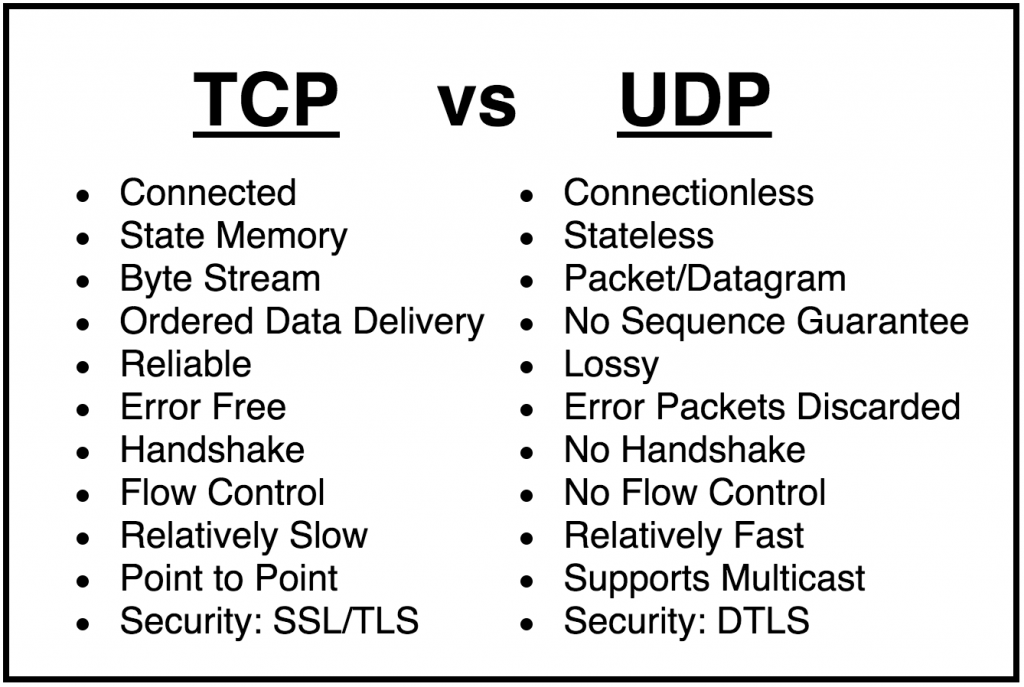
\includegraphics[scale=0.5]{TCP-vs-UDP}
	\caption{Comparison between TCP and UDP protocols, from \cite{NetBurner:TCP-vs-UDP}}
\end{figure}


\section{Custom transport implementation}
While TCP and UDP are great at solving their own use-cases, there exists a major problem: each protocol solves only one type of transparency. With the rise of online gaming, there appeared the need for having both transparency implementations at once; some data would require reliability and ordering that TCP provides (for example, textual chat messages), while other types needed only latest data without the guarantee of delivery (for example, position of the player in a virtual world). \\

Using both protocols at the same time, based on the type of data, is not an ideal solution either, for multiple reasons \cite{GafferOnGames:UDP-vs-TCP}:

\begin{enumerate}
	\item Using TCP can induce packet loss in UDP packets as routers often prioritize TCP segments (as dropping TCP segment requires re-sending, while dropping UDP packet does not).
	\item Supporting many reliable channels (for example, one channel for text message data, another for images or audio) would require many TCP connections, quickly exhausting operating system resources.
	\item Application code-base would be hard to manage, potentially resulting in slower development and harder to track bugs.
\end{enumerate}

For all of those reasons, a custom solution is required - one that allows the user to easily specify, on per packet basis, how data should be delivered. If data is time-sensitive, user must be able to send it in unreliable manner, where temporal transparency is preserved. If data is important and must be delivered, semantic transparency must be preserved. As UDP already provides temporal transparency, we simply need to upgrade it with optional semantic transparency features that are present in the TCP. Implementations of such protocols are often called RUDP - \textit{Reliable User Datagram Protocol}. The rest of this chapter explains one such implementation.



\subsection{Packet}
\classname{Packet} represents a single outgoing message of arbitrary data that can be sent over the network. It is a thin abstraction layer over raw byte-array and therefore offers some of the benefits that a raw byte-array cannot. \\

One such benefit is object pooling\footnote{https://en.wikipedia.org/wiki/Object\_pool\_pattern}. As creation of packets is a very frequent occurrence in networked applications, allocating new packet instances (which also internally keeps a medium sized byte-array) each time a packet is needed would quickly fill-up heap memory, prompting execution of garbage collection\footnote{https://en.wikipedia.org/wiki/Garbage\_collection\_(computer\_science)}. This is especially important in applications that have time constraints, such as games, where even one slowly executed frame could ruin user experience. \\

Another benefit is separation of write-only and read-only operations. Since \classname{Packet} represents an outgoing packet, it only offers methods for writing data (constructing the packet). Those methods also provide powerful functionality, allowing user to construct packets containing complex structures. \\

\begin{figure}[h!]
	\centering
	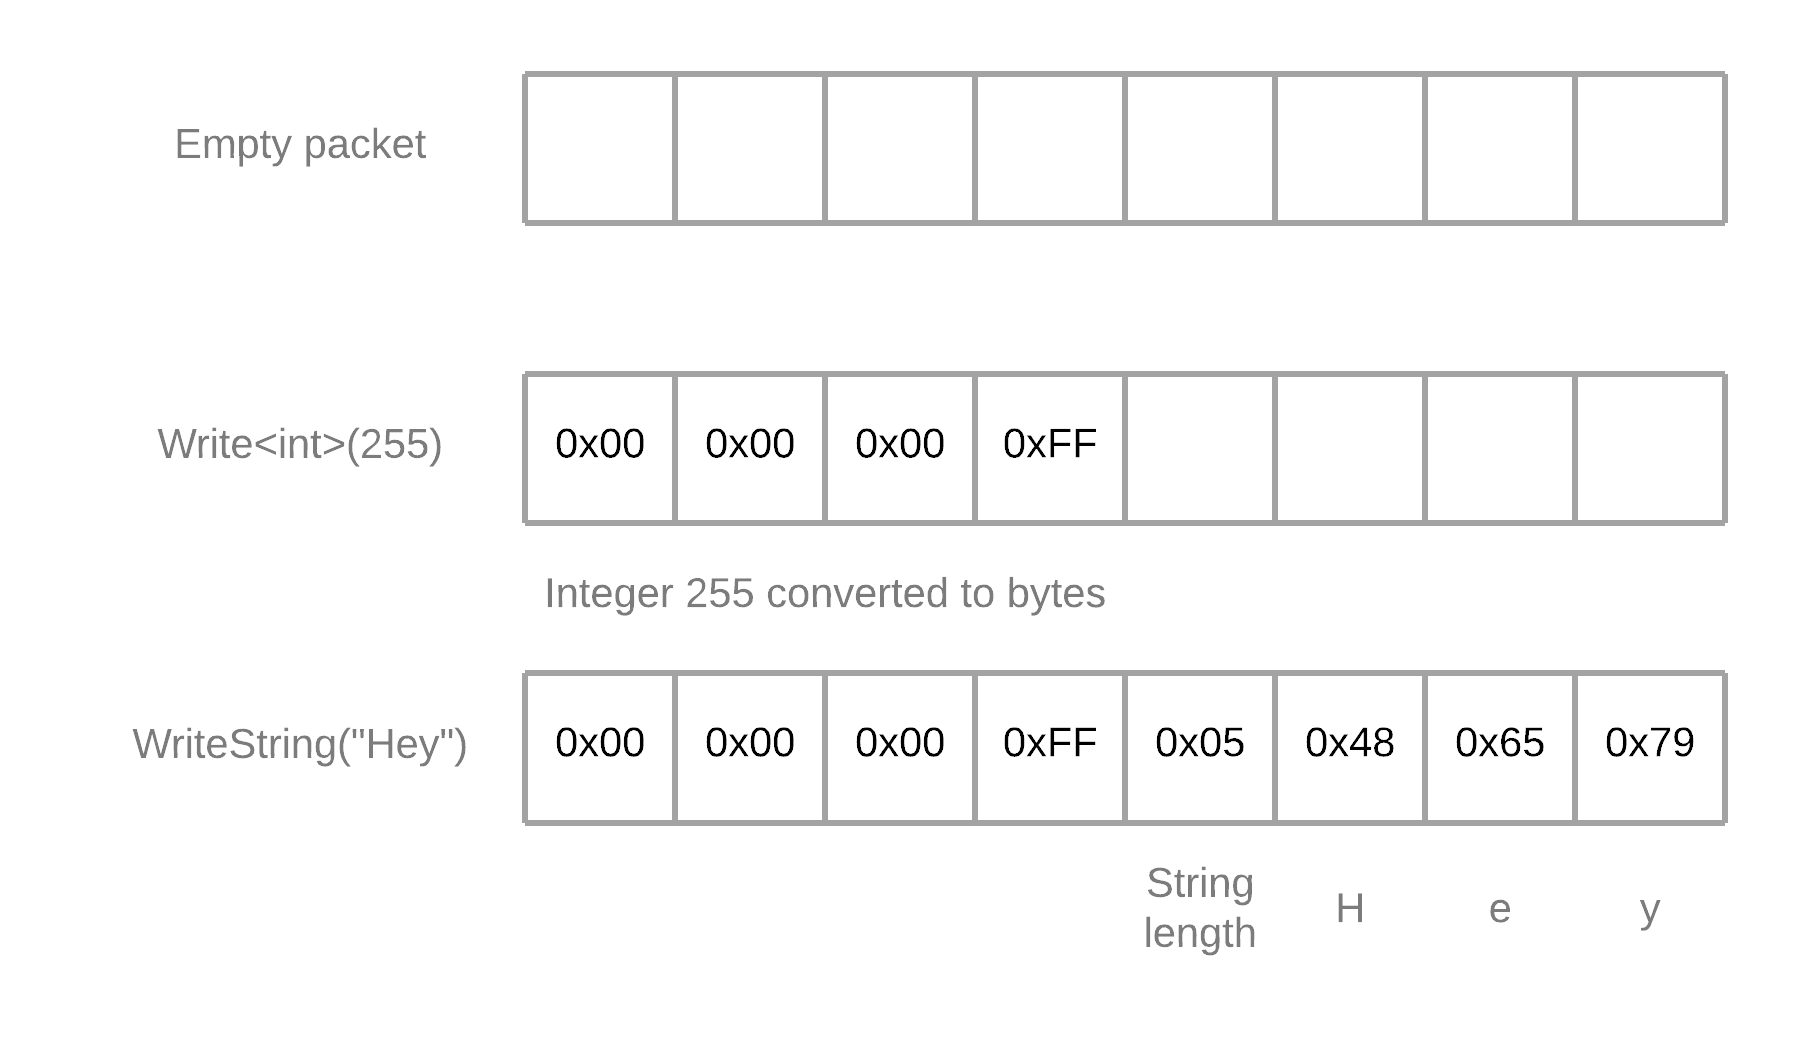
\includegraphics[scale=0.22]{Packet-write}
	\caption{Example of writing data to a packet}
\end{figure}

Similarly to \classname{Packet}, which is write-only, there exists a read-only packet version named \classname{Read\-Only\-Packet} which represents a single incoming message of arbitrary data that was received over the network. It offers the same interface as \classname{Packet}, but instead of write, read methods are exposed. Another important feature of \classname{Read\-Only\-Packet} is that it cannot in any way modify underlying packet data, making it very safe to use, even in multi-threaded scenarios. \\

Finally, the last benefit is cleaner code. Spotting an instance of \classname{Packet} or \classname{Read\-Only\-Packet} immediately gives information to the reader that this code works with networking. Same could not be said for byte-array as its usages are much broader. \\

\classname{Packet} also defines an important constant, which is the maximum size, in bytes. This constant is carefully chosen to avoid packet fragmentation on the network layer. Any packets that require bigger size must use a fragmented channel which will perform fragmentation and reassembly on the application layer. Maximum size is equal to Ethernet MTU (Maximum transmission unit, 1500 bytes) subtracted by IP header size (20 bytes) and UDP header size (8 bytes), which results in maximum size of 1472 bytes.\\

\begin{equation}
	Maximum \; size = 1500 - 20 - 8 = 1472 \; bytes \label{eq:max_packet_size}
\end{equation}

\subsubsection{Packet structure}
Each packet follows the same structure, which is a header type followed by the header-specific payload. It is important to mention that header is always inserted as the first byte without any exceptions.

\begin{figure}[h!]
	\centering
	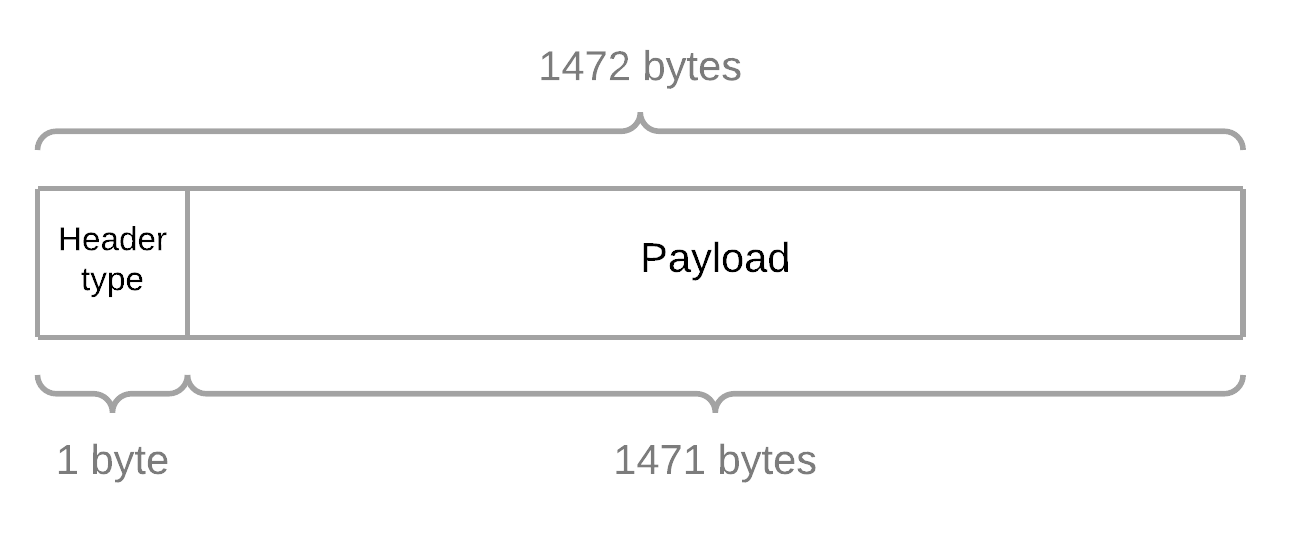
\includegraphics[scale=0.25]{Packet-structure}
	\caption{Packet structure}
\end{figure}


\subsubsection{Header types}
Header type is used to denote what kind of packet it is and allows the receiver to decode the meaning behind received bytes.

\begin{table}[H]
	\centering
	\resizebox{\textwidth}{!}{%
		\begin{tabular}{|c|c|c|}
			\hline
			\textbf{Header type} & \textbf{Description}                                                                                                                   & \textbf{Payload}                                                                       \\ \hline
			Connect              & \begin{tabular}[c]{@{}c@{}}Sent by the client to server when\\ establishing a virtual connection.\end{tabular}                         & Optional connect data                                                                  \\ \hline
			ConnectApproved      & \begin{tabular}[c]{@{}c@{}}Sent by the server to client when\\ connection request has been approved.\end{tabular}                      & -                                                                                      \\ \hline
			Ping                 & \begin{tabular}[c]{@{}c@{}}Used for measuring connection latency\\ and serves as a keep-alive packet.\end{tabular}                     & Sequence number                                                                        \\ \hline
			Pong                 & Response to the ping packet.                                                                                                           & Sequence number                                                                        \\ \hline
			Data                 & Indicates that the packet contains data.                                                                                               & \begin{tabular}[c]{@{}c@{}}Channel ID, channel header,\\ application data\end{tabular} \\ \hline
			Acknowledgement      & \begin{tabular}[c]{@{}c@{}}Indicates that specific set of\\ packets have been received.\end{tabular}                                   & \begin{tabular}[c]{@{}c@{}}Channel ID, sequence number,\\ ack bit-field\end{tabular}   \\ \hline
			Disconnect           & \begin{tabular}[c]{@{}c@{}}Sender has closed its side of the connection and\\ will no longer send or receive any packets.\end{tabular} & -                                                                                      \\ \hline
			Timeout              & Indicates that a connection has timed-out.                                                                                             & -                                                                                      \\ \hline
		\end{tabular}%
	}

	\caption{All of the possible header types.}
	\label{table:header-types}
\end{table}

Only one header type is special, and that is the \textit{Data} type, as that is the only type with which the end-user is going to interact with.

\begin{figure}[h!]
	\centering
	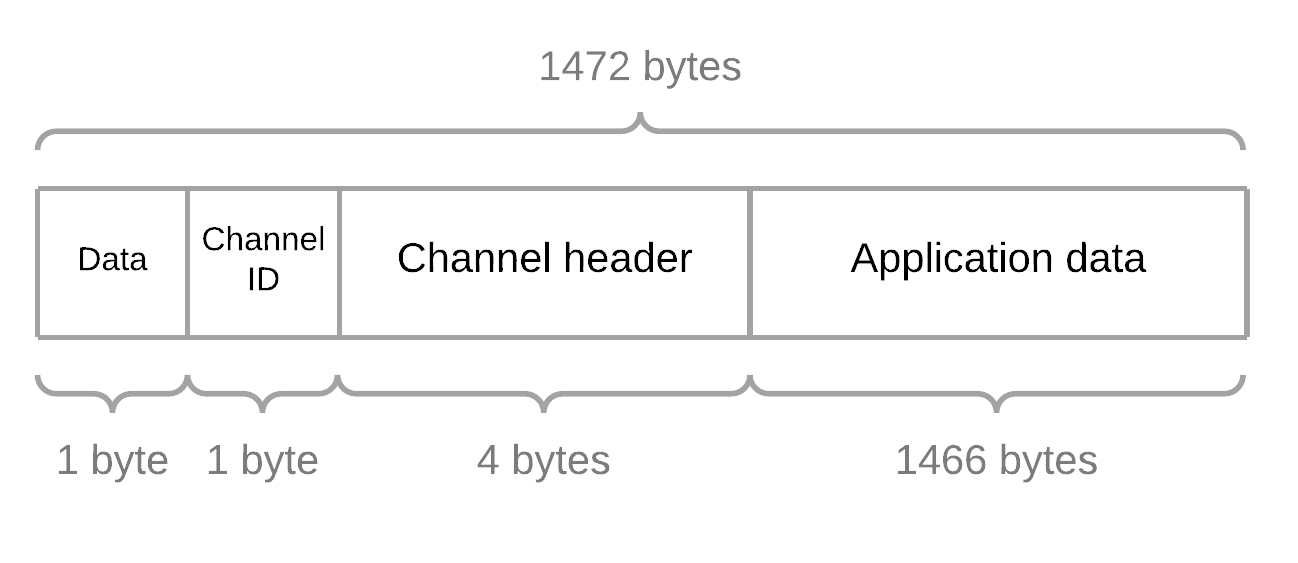
\includegraphics[scale=0.2]{Data-packet-structure}
	\caption{Data-packet structure}
\end{figure}


\subsection{Array pooling}
Fluid gameplay with no stuttering is essential for user experience. Standard value that always needs to be maintained is at least 60 frames per second\footnote{https://en.wikipedia.org/wiki/Frame\_rate} (FPS). Failing to render at least that many frames each second is going to result in noticeable lag, drastically decreasing overall user satisfaction. This constraint means that all of the updates need to be performed in about 16 milliseconds. Consequently, this implies that expensive, long-running operations should be run as rarely as possible. One such operation is the process of garbage collection\footnote{https://en.wikipedia.org/wiki/Garbage\_collection\_(computer\_science)}, where all of the previously allocated memory that is no longer referenced is being freed.\\

However, garbage collection is only triggered when memory is no longer referenced. If we keep a reference to previously allocated memory and reuse it, no garbage collection will be performed. Such process of reusing memory is called \textit{object pooling}\footnote{https://en.wikipedia.org/wiki/Object\_pool\_pattern} and is a standard practice in high-performance applications. As networked applications constantly keep sending packets back and forth (and packets are essentially just arrays of bytes), utilizing object pooling is perfectly suitable.\\

In our implementation, array pooling is implemented using an array of buckets. In this context, term \textit{bucket} means a collection of reusable arrays. Each bucket holds multiple arrays of same sizes and each subsequent bucket holds arrays of exponentially increasing capacities. First bucket holds arrays of size \textit{Packet.MaxSize}. Last bucket holds arrays of sizes \textit{Packet.MaxSize * 256}, which is maximum allowed size of a fragmented packet.


\begin{figure}[h!]
	\centering
	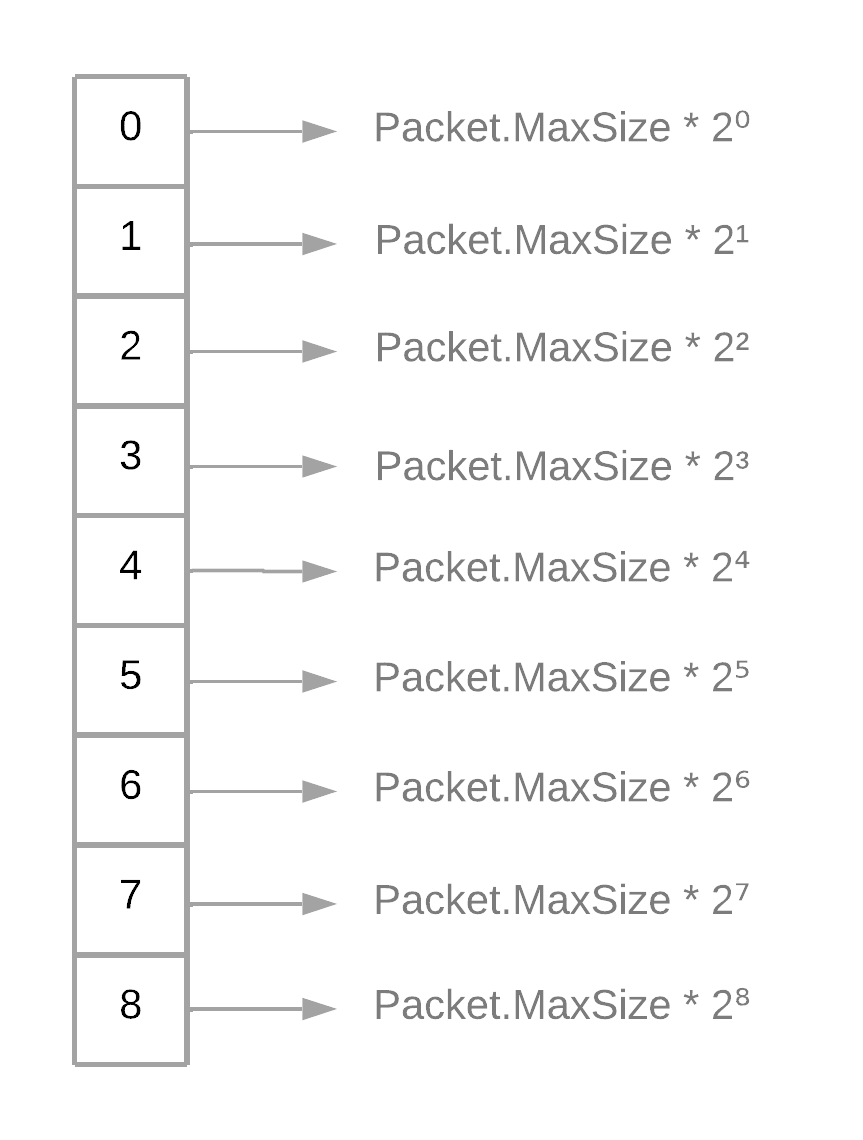
\includegraphics[scale=0.2]{Array-pool-buckets}
	\caption{Array pool buckets}
\end{figure}



\subsection{Channels}
Channel represents a component that controls the way packets are sent and received. There are four fundamental problems that a channel can, but does not have to solve:

\begin{enumerate}
	\item \textbf{Order} - ability for the receiver to receive packets in order in which they were originally sent.
	\item \textbf{Duplication} - ability for receiver to detect and discard duplicate packets.
	\item \textbf{Reliability} - ability for sender to ensure that receiver received a packet.
	\item \textbf{Fragmentation} - ability for sender to divide a big packet into smaller packets called \textit{fragments} and for receiver to reassemble those into original big packet.
\end{enumerate}

\begin{center}
	\begin{table}[H]
		\centering
		
		\begin{tabular}{ |c|c|c|c|c|c| } 
			\hline
			Name & Order & Duplication & Reliability & Fragmentation \\ 
			\hline
			Unreliable        & - & - & - & - \\ 
			Sequenced         & Yes & Yes & - & - \\ 
			Reliable          & Yes & Yes & Yes & Yes \\ 
			\hline
		\end{tabular}
		
		\caption{Channel implementations and problems each implementation solves}
	\end{table}
\end{center}

Each channel also has a name associated with it and keeps track of bandwidth statistics, which is useful for diagnosing network usage. Information tracked by the channel are following state variables:

\begin{enumerate}
	\item \textbf{Packets sent} represents total number of packets sent through the channel.
	\item \textbf{Bytes sent} represents total number of bytes sent through the channel.
	\item \textbf{Packets received} represents total number of packets received on the channel.
	\item \textbf{Bytes received} represents total number of bytes received on the channel.
\end{enumerate}



\subsubsection{Unreliable channel}
Unreliable channel is the most basic channel type that does no processing of sent and received packets. Since it does not perform any logic, this channel type does not use any header bytes in the packet. It acts as a pure UDP socket, therefore it does not provide any insurance:

\begin{enumerate}
	\item Packets can arrive out-of-order and receiver has no way of reassembling packets in order.
	\item Packets can be duplicated in the network and receiver has no way of knowing it received a duplicate packet.
	\item Packets can be lost in the network and sender has no way of knowing if packet was potentially lost in transit.
	\item Packet size is limited as there is no support for fragmentation and reassembly.
\end{enumerate}

\begin{figure}[h!]
	\centering
	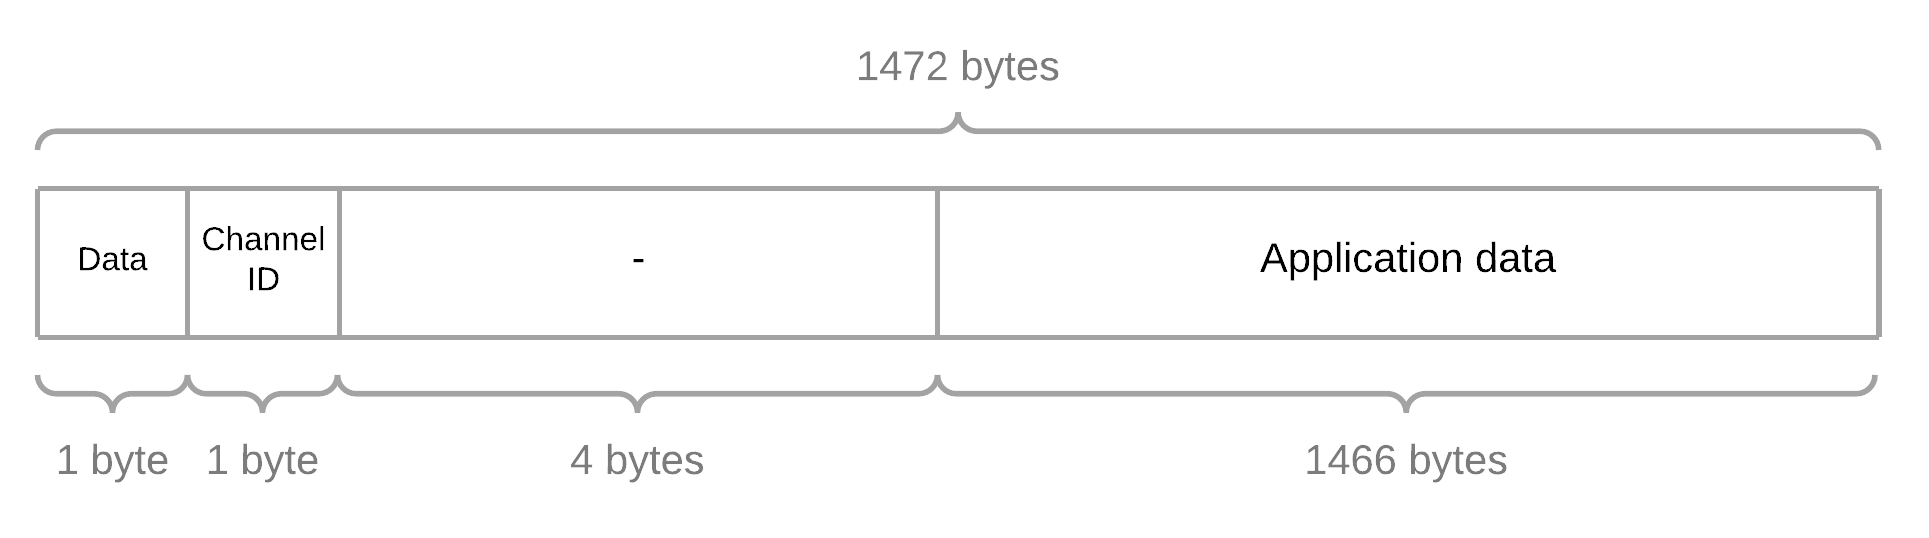
\includegraphics[scale=0.2]{Unreliable-packet-structure}
	\caption{Format of the packet sent through the unreliable channel.}
\end{figure}



\subsubsection{Sequenced channel}
Sequenced channel solves two problems: order and duplication. It does so by attaching a unique number to each outgoing packet called \textit{local sequence number}, which is a state variable maintained by the sending side of the channel. For each packet sent, local sequence number is incremented.

\begin{figure}[h!]
	\centering
	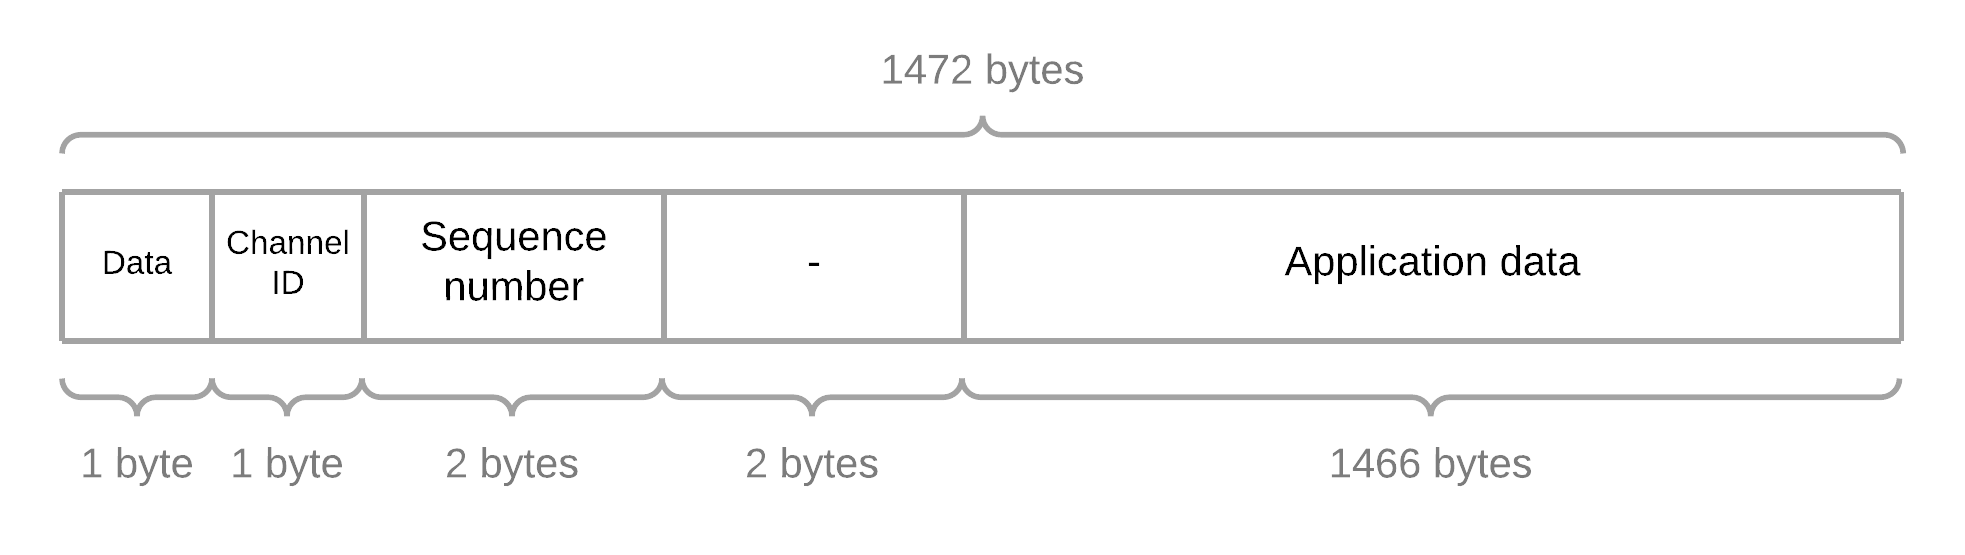
\includegraphics[scale=0.2]{Sequenced-packet-structure}
	\caption{Format of the packet sent through the sequenced channel.}
\end{figure}

On the receiver side, another state variable is maintained: \textit{remote sequence number}. The remote sequence number holds the value of the highest received sequence number and this value is used to determine whether a newly received packet should be accepted or discarded. \\

Once a new packet is received, the sequence number is read from the packet. If the sequence number contained in the packet is greater than the remote sequence number, packet is accepted, otherwise it is discarded. \\

Another problem needs to be addressed: sequence number wrapping. As sequence numbers are stored in only 2 bytes, maximum sequence number value can be 65535. Once this sequence number is reached, next packet sequence number is going to wrap back to the minimum value of 0. Using naive approach of comparing raw sequence number values is going to produce wrong results; even though 65535 is numerically greater than 0, it logically is not. To solve this problem, the following algorithm is used to compare sequence numbers:

\begin{algorithm}[H]
	\caption{Comparing sequence numbers with wrapping}
	\textbf{Input:} First sequence number $seq1$, second sequence number $seq2$ \\
	\textbf{Output:} $true$ if $seq1$ is greater than $seq2$, $false$ otherwise \\
	
	\begin{algorithmic}
		\State $isGreaterRegular \gets seq1 > seq2 \And seq1 - seq2 \leq 32767$
		\State $isGreaterWithWrap \gets seq1 < seq2 \And seq2 - seq1 > 32767$ \\
		\Return $isGreaterRegular \Or isGreaterWithWrap$
	\end{algorithmic}
\end{algorithm}

Algorithm is based on a simple idea: if sequence number values are close numerically, wrapping did not occur. Sequence numbers are close if absolute value of their difference is smaller or equal to half of the full sequence number range.



\chapter{Uvod}
Uvod rada. Nakon uvoda dolaze poglavlja u kojima se obrađuje tema.

\chapter{Zaključak}
Zaključak.

\bibliography{literature}
\bibliographystyle{fer}

\begin{sazetak}
Sažetak na hrvatskom jeziku.

\kljucnerijeci{Ključne riječi, odvojene zarezima.}
\end{sazetak}

\engtitle{Development and application of a videogame multiplayer networking library}
\begin{abstract}
Abstract.

\keywords{Keywords.}
\end{abstract}

\end{document}
